\documentclass[a4paper]{article}
\usepackage[utf8]{inputenc}
\usepackage[catalan]{babel}
% No tocar l'odre del que hi ha amunt.

% Lletres romanes
\usepackage{amsmath}

% paquet per a fer boniquet
\usepackage{fancyhdr}
\pagestyle{fancy}
\fancyhf{}
\fancyhead[RE, RO]{\textbf{German.. i Sistach}}
\fancyhead[LE, LO]{Sistemes Operatius $\textup{\uppercase\expandafter{\romannumeral 2}}$}
% Fi boniquet

% Per introduir .eps "taula del abre per exemple", el odre te importància
\usepackage{graphicx}
\usepackage{epstopdf}

% Per poder posar codi
\usepackage{listings}

\author{Arnau Sistach Reinoso}
\title{Pràctica 1}
\begin{document}
\maketitle
\tableofcontents
\newpage

\section{Seguint el guió}

Farem el que indica l'enunciat per a tenir la pràctica llesta.

\subsection{Lectura i extracció de dades del fitxer}

Hem compilat el codi, hem comprovat que el codi funciona correctament amb \textbf{valgrind}.
També hem modificat el valor del \textbf{MAXCHAR} a 10, però a la nostra sorpresa, el \textbf{valgrind} no dona cap error i la sortida és la mateixa.

Hem canviat el \textbf{MAXCHAR} a 128, ja que hi ha línies de 102 caràcters. Per evitar problemes ens hem curat en salut.
I finalment hem comprovat que amb el \textbf{valgrind} funciona tot correctament.

\subsection{Inserció de l'origen a l'abre binari}
Ens dona un error. Ara toca descobrir a on:
\begin{figure}[h]
\centering
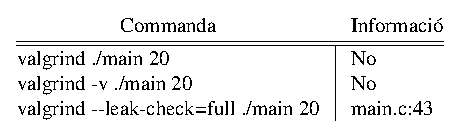
\includegraphics{1Entrega/tblAbre.eps}
\end{figure}

On la línia 43 és:

\begin{lstlisting}[language=C]
  /* Allocate memory for tree */
  tree = (RBTree *) malloc(sizeof(RBTree));
\end{lstlisting}

Ara, per a solucionar-ho, editarem la funció:
\begin{lstlisting}[language=C]
  /* Delete the tree */
  deleteTree(tree);
\end{lstlisting}

Problema resolt.


Ara tenim un problema, l'enunciat diu que només hem de fer cas als que tenen una llargada de 3!
Llavors això implicarà que sempre ens tocarà fer un free.

\subsection{Inserció del destí a la llista enllaçada}

Hem comprovat que el \textbf{valgrind} no dona cap error.
Tot i que aquí ho resolt el main, hem preferit fer-ho automaticament al cridar:
\begin{lstlisting}[language=C]
  /* Delete the list */
  deleteList(list);
\end{lstlisting}

\section{Sense el guió}

FALLA
\begin{lstlisting}[language=C]
token = strtok ( line, "," );
for ( i = 0; (i < AIR_COLUMN) && token; i++ )
{
	strcpy ( all[i], token );
	token = strtok ( NULL, "," );
}
\end{lstlisting}


Canviat i funciona!
\begin{lstlisting}[language=C]
do
{
	c = line[i++];
	if ( c == ',' )
	{
		line[i -1] = '\0';
		v[j++] = line + i;
	}
} while ( c );
\end{lstlisting}


\end{document}
